
\documentclass{avocado}
\usepackage[toc,page]{appendix}


\usepackage[ngerman]{babel}
\usepackage[german=quotes]{csquotes}
\usepackage{float}
%\usepackage{bibgerm}
\usepackage{amsmath}
\usepackage{tabularx}
\usepackage{graphicx}
\usepackage{pdflscape}
\usepackage{xstring}
\usepackage{caption}
\usepackage[backend=biber, style=ieee]{biblatex}
\usepackage{pgfplots}
\usepackage{pgfgantt}
%\usepackage{ltablex} % breaks the history tabularx


\addbibresource{sources.bib}
%\usepackage[fixlanguage]{babelbib}
%\selectbiblanguage{german}
%\bibliographystyle{ieeetr}
%\addbibresource{sources}
\newcommand{\mail}[1]{\href{mailto:#1}{#1}}
\setlength{\parindent}{0cm}

\newcommand{\titel}{Avocado Share}
\newcommand{\shorttitel}{}
\newcommand{\doctype}{Projektplanung}
\newcommand{\untertitel}{Studentenplattform zum Know-How-Transfer}
\newcommand{\datum}{\today}
\newcommand{\team}{Gruppe 13}
\newcommand{\autorA}{Bergmann Sascha}
\newcommand{\autorB}{Kunz Lion}
\newcommand{\autorC}{Ngueyen Dang Thien}
\newcommand{\autorD}{Müller Cyril}
\newcommand{\autorE}{}
\newcommand{\ort}{Winterthur}
\newcommand{\dozent}{}
\newcommand{\betreuer}{}
\newcommand{\version}{0.1}

\hypersetup{
    bookmarks=false,    % show bookmarks bar?
    pdftitle={\titel - \doctype},    % title
    pdfauthor={\autorA, \autorB, \autorC, \autorD},  % author
    pdfsubject={Funktionale und nicht-funktionale Anforderungen}, % subject of the document
    pdfkeywords={\titel, \doctype, \team, Version \version, PSIT, IT15b}, % list of keywords
    colorlinks=true,        % false: boxed links; true: colored links
    linkcolor=blue!30!black,% color of internal links
    citecolor=black,        % color of links to bibliography
    filecolor=black,        % color of file links
    urlcolor=black,         % color of external links
    linktoc=page            % only page is linked
}%

%\project{Avocado Share}
\title{\title}
\author{\autorA \and \autorB \and \autorC \and \autorD \and \autorD}

\newcommand{\user}[1]{$U_#1$}
\newcommand{\group}[1]{$G_#1$}

\usepackage[toc, xindy]{glossaries}
%\newglossary[glignoredl]{ignored}{glignored}{glignoredin}{Ignored Glossary}

\makeglossaries

\begin{document}
% title page -------------------------------------------------------------------
\thispagestyle{plain}

\begin{titlepage}
    \begin{flushleft}
        \vspace*{1cm}
        \textbf{
            \hspace{-0.12cm}\LARGE{\doctype}\\
            \Huge{\titel}\\
            \vspace{0.5cm}
            \large{\untertitel}\\
            \vspace{1.5cm}
            \large{\team\\}
        }
            \large{\autorA, \autorB,\\\autorC, \autorD}\\
        \vspace{1cm}
        \vfill
        \large{
            \iffalse % We don't need a dozent or a betreuer
                \hspace{-0.83cm} \includegraphics{images/zhaw_logo_full}\\
                \line(1,0){165} 

                \vspace{0.5cm}
                Auftraggeber:\\ \dozent \\
                Betreuer:\\ \betreuer \\
                \vspace{0.5cm}
            \fi
            \ort, \datum \hfill Version: \version
        }
    \end{flushleft}
\end{titlepage}
% end of titlepage -------------------------------------------------------------
\section*{Dokumentenhistorie}
\begin{tabularx}{\linewidth}{|l|r|X|} \hline
Version & \multicolumn{1}{l|}{Datum} 			& Anpassungen \\ \hline
0.1 & 05.12.2015 & Dokumentstruktur und erster Entwurf \\ \hline
0.2 & 06.12.2015 & Überarbeitung des Inhaltes und der Diagramme \\ \hline
\end{tabularx}

\clearpage

%\vfill
\section*{Unterschriften}
\begin{minipage}[t][5cm][t]{0.45\linewidth}
\subsection*{Auftraggeber}
Prof. Dr. Max Lemmenmeier \\
ZHAW, Dept. Linguistik \\
%LCC Language Competence Centre \\
%Büro SF 03.09 \\
Theaterstr. 17 \\
%Postfach \\
8400 Winterthur \\
%Tel. 0041 58 934 60 73 \\
\mail{max.lemmenmeier@zhaw.ch} \\
\vfill \hrule
\end{minipage} \hfill
\begin{minipage}[t][5cm][t]{0.45\linewidth}
\subsection*{Auftragnehmer}
Leiter Projektgruppe \\
Sascha Bergmann \\
ZHAW, Bachelorstudent ICT \\
\mail{bergmsas@students.zhaw.ch} \\
\vfill \hrule
\end{minipage} \\
%\begin{minipage[t]{0.45\linewidth}
%\subsection*{Auftraggeber}
%\end{minipage}
\clearpage

\tableofcontents
\clearpage
\section{Einleitung}
Die Projektplanung ist ein wichtiger Bestandteil des Projektmanagements. 
In diesem Dokument wird ein Grundstein gelegt, um eine genaue Termin- und Aufwandplanung des Projektes
zu ermöglichen. 
Die Anforderungen, wie sie im Pflichtenheft beschrieben sind, wurden in Arbeitspaketen gegliedert, welche
im Laufe der nächsten Projektphasen ausgeführt werden. Im Netzplan werden diese Pakete graphisch dargelegt.
Zusätzlich zeigt dieses Dokument sowohl den gesamten Aufwand, als auch die Auslastung der einzelnen Teammitglieder auf.

\section{Netzplan}
Im folgenden Netzplan sind alle Arbeitspakete der Entwicklung des Avocado-Share dargestellt. 
Um sicherzustellen, dass jedes Arbeitspaket termingerecht und vollständig ausgeführt wird, haben wir beschlossen, neben dem Verantwortlichen auch eine Person zu bestimmen, welche eine Aufgabe ausführt.\\

Durch eine Planungsphase zu Beginn des Projektes, ist es uns möglich eine klare Schichtentrennung zu machen.
Da wir in der Planung die Schnittstellen zwischen den Schichten definieren, ist es uns möglich die Entwicklungsschritte danach
alle parallel auszuführen. Dadurch erhalten wir zwar einen kleinen Flaschenhals beim Erstellen der Grobstruktur und des
Grundgerüstes, doch es bringt uns viel Freiheit in den folgenden Paketen. So können wir besser und einfacher auf allfällige
Verzögerungen und Ausfälle reagieren.
Da wir eine technisch saubere Lösung haben wollen, ist es uns wichtig, dass die Spezialisten eines Bereiches in unserem Team auch entweder Verantwortlicher oder Ausführender eines Arbeitspaketes sind. \\

In jedem Arbeitspaket inbegriffen ist, wo sinnvoll, auch das Testing.
Bei Arbeitspaketen in welchen Java-Code geschrieben wurde, sollten Unit-Tests geschrieben werden.
Bei Web- und UI-Paketen sollte ein kurzes Test-Protokoll geschrieben werden, um sicherzustellen, dass alle Funktionen auch korrekt funktionieren.
So kann beim Arbeitspaket Testing schnell und einfach alles nochmals getestet werden.\\

Design- und Planungspakete haben als "`Test"' ein Review mit dem gesamten Team.

\begin{landscape}
% \vspace*{\fill}: center vertically 
% source: https://stackoverflow.com/questions/3141702/vertically-centering-a-title-page
\vspace*{\fill}
\begin{figure}[H]
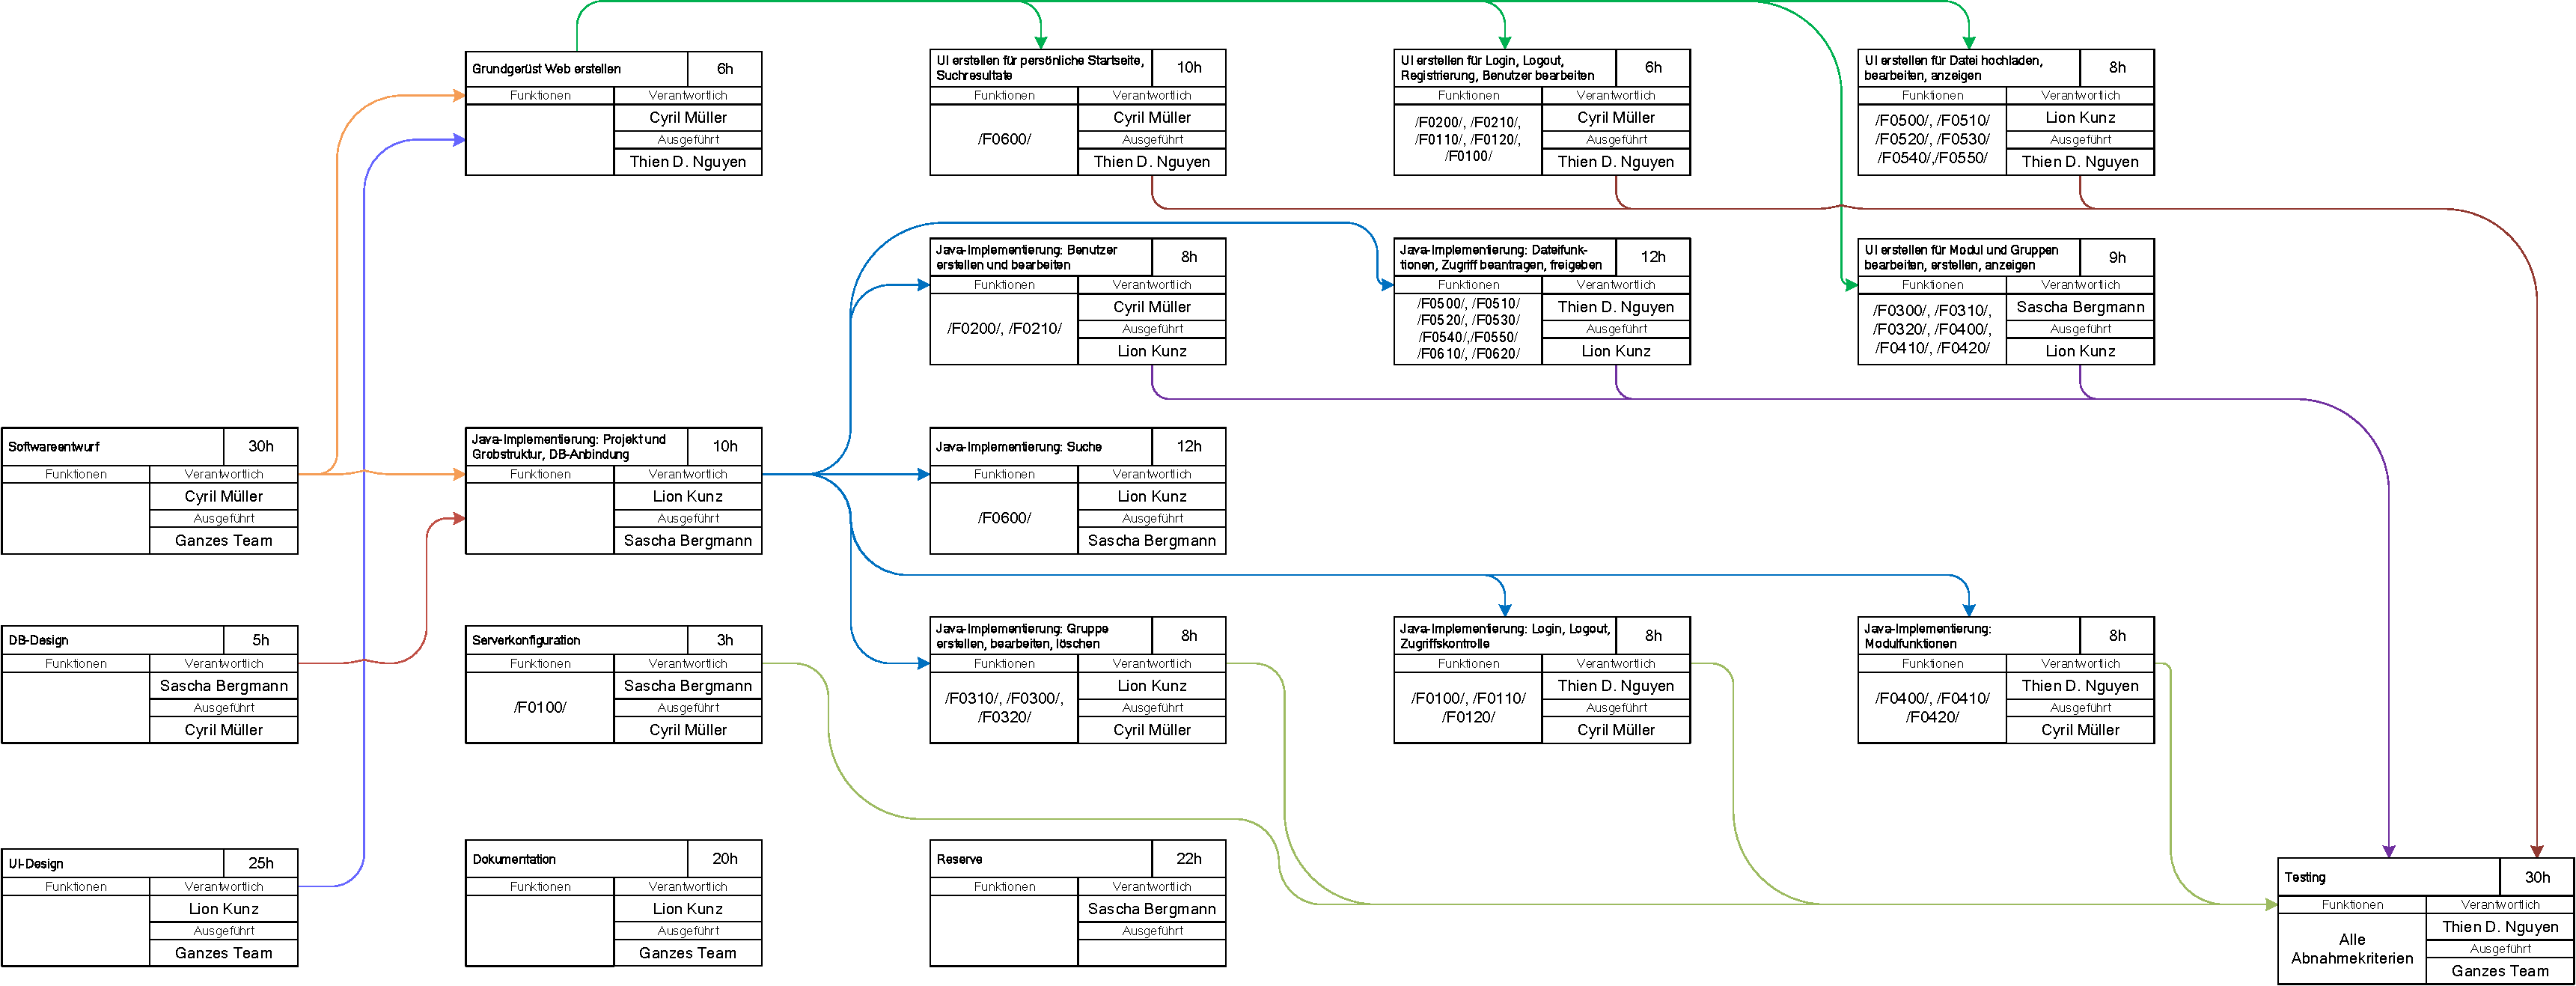
\includegraphics[width=\linewidth]{graphics/netzplan_s2.pdf}
\caption{Der Netzplan zeigt die Arbeitspakete, geordnet nach Arbeitsprozessen.}
\end{figure}
\vspace*{\fill}
\end{landscape}

\section{Ressourcenplanung}
\subsection{Meilensteine}
Unser Team hat sich darauf geeinigt, dass der Projektleiter über die gesamte Zeit bei derselben Person bleibt.
So ist immer klar wer den Überblick haben muss und es gibt keine Wissens-Verluste bei der Übergabe des Projektstandes zwischen Projektleitern. 

\begin{tabularx}{\textwidth-2cm}{|l|l|X|} \hline
\textbf{Meilenstein}	& \textbf{Verantwortlichkeit} &	\textbf{Erwartung} \\ \hline
\textbf{M1}	&Sascha Bergmann	&Vorschau GUI, Datenbank (ER-Schema) \\  \hline
\textbf{M2}	&Sascha Bergmann	&Design und DB umgesetzt; mind. Ein Hauptprozess vollständig umgesetzt \\ \hline
\textbf{M3}	&Sascha Bergmann	&Hauptprozesse umgesetzt; Codierungsstil/Modularisierung \\ \hline
\textbf{M4}	&Sascha Bergmann	&Abnahmetests; Gruppenspezifischer Schwerpunkt \\ \hline
\textbf{M5}	&Sascha Bergmann	&Präsentation der Arbeit \\ \hline
\end{tabularx}

\iffalse
  \begin{ganttchart}{1}{12}
    \gantttitle{Projektplan}{12} \\
    \gantttitlelist{1,...,12}{1} \\
    \ganttmilestone{Meilenstein M1}{4}  \ganttnewline
    \ganttmilestone{Meilenstein M2}{5}  \ganttnewline
    \ganttmilestone{Meilenstein M3}{6}  \ganttnewline
    \ganttmilestone{Meilenstein M4}{7} 
  \end{ganttchart}
\fi

\subsection{Auslastung}
Die Auslastung ist bei allen Personen sehr ähnlich. Der Projektleiter Sascha Bergmann hat ein paar Stunden weniger als die anderen Teammitglieder. Dies ist absichtlich so gelöst, da der Projektleiter noch Zeit benötigt administrative Arbeiten auszuführen, wie z.B. Vorbereitung von Meilenstein-Sitzungen, Arbeitsstände überprüfen, eventuelle Planungsänderungen vornehmen.

\definecolor{bergmansas}{HTML}{5B9BD5}
\definecolor{kunzlio}{HTML}{ED7D31}
\definecolor{muellcy1}{HTML}{A5A5A5}
\definecolor{nguyeda}{HTML}{FFC000}

\begin{figure}[H]
\centering
\pgfplotstableread{
MS    bergmansas     kunzlio    muellcy1    nguyeda
1     13.75          13.75      18.75       13.75
2     10             12         11          20
3     12             17         16          10
4     12.5           12.5       12.5        12.5
}\datatable

\begin{tikzpicture}
\begin{axis}[
	width=\linewidth-2cm,
	xbar stacked,
	area legend,
	ytick=data,
	yticklabels={Aufwand M1,
				Aufwand M2,
				Aufwand M3,
				Aufwand M4,
				%\emph{Total}
				},
	legend style={
		legend columns=2,
		at={(xticklabel cs:0.5, 20)},
		anchor=north,
		draw=none
	},
	xlabel={Aufwand in Stunden},
	xticklabel pos=lower,
	minor x tick num=1,
	xmin=0,
	xmax=65,
	bar width=4mm,
	y=7.5mm,
	enlarge x limits={abs=0},
	enlarge y limits={abs=0.7},
	grid=major,
	y dir=reverse,
    point meta=explicit,
    %calculate offset/.code={
    %    \pgfkeys{/pgf/fpu=true,/pgf/fpu/output format=fixed}
    %    \pgfmathsetmacro\testmacro{(\pgfplotspointmeta*10^\pgfplots@data@scale@trafo@EXPONENT@x)/2*\pgfplots@x@veclength)}
    %    \pgfkeys{/pgf/fpu=false}
    %},
    %every node near coord/.style={
    %    /pgfplots/calculate offset,
    %    yshift=-\testmacro
    %},
	%nodes near coords,
	%nodes near coords align=center
]
\addplot[bergmansas,fill=bergmansas] table [y={MS}, x=bergmansas] \datatable;
\addplot[kunzlio,fill=kunzlio] table [y={MS}, x=kunzlio] \datatable;
\addplot[muellcy1,fill=muellcy1] table [y={MS}, x=muellcy1] \datatable;
\addplot[nguyeda,fill=nguyeda] table [y={MS}, x=nguyeda] \datatable;
\legend{S. Bergmann, L. Kunz, C. Müller, D. Nguyen}
\end{axis}
\end{tikzpicture}
\caption{Auslastung pro Meilenstein.}
\end{figure}



\begin{figure}[H]
\centering
\begin{tikzpicture}
\centering
\begin{axis}[
	width=\linewidth-2cm,
	xbar stacked,
	area legend,
	ytick=data,
	yticklabels={S. Bergmann,
				L. Kunz,
				C. Müller,
				D. Nguyen,
				\emph{Total}
				},
	xlabel={Aufwand in Stunden},
	xticklabel pos=lower,
	minor x tick num=1,
	xmin=0,
	xmax=65,
	bar width=4mm,
	y=7.5mm,
	enlarge x limits={abs=0},
	enlarge y limits={abs=0.7},
	grid=major,
	y dir=reverse
]
\addplot[bergmansas,fill=bergmansas, x={label}, y={bergmansas}] coordinates
% Transfer
{%(13,0)
(48.25, 0)
(0,1)
(0,2)
(0,3)
};

\addplot[kunzlio,fill=kunzlio] coordinates
{
(0,0)
(55.25,1)
(0,2)
(0,3)
};

\addplot[muellcy1,fill=muellcy1] coordinates
{
(0,0)
(0,1)
(58.25,2)
(0,3)
%(18.75,0)
%(11,1)
%(16,2)
%(12.5,3)
%(,4)
};

\addplot[nguyeda, fill=nguyeda] coordinates
{
(0,0)
(0,1)
(0,2)
(56.25,3)
%(,4)
};

%\legend{Sascha Bergmann, Lion Kunz, Cyril Müller, Dang Thien Nguyen}

\end{axis}
\end{tikzpicture}
\caption{Gesamte Auslastung pro Person.}
\end{figure}

\begin{figure}[H]
\centering
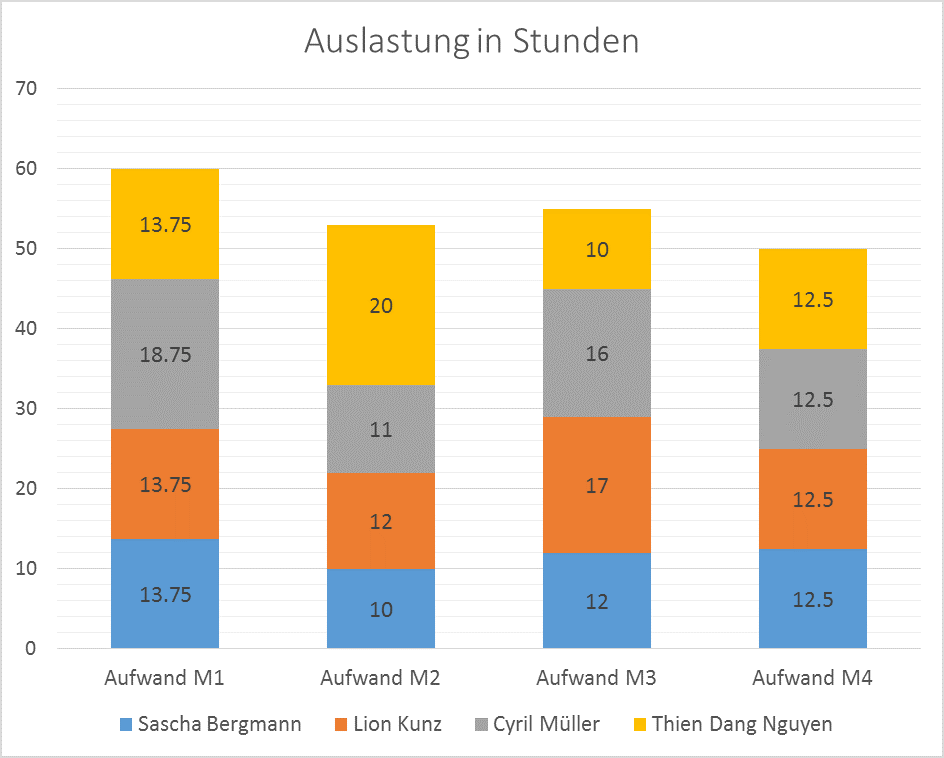
\includegraphics[width=0.7\textwidth]{graphics/auslastung_meilensteine.png}
\caption{Aufwand pro Meilenstein.}
\end{figure}


\begin{figure}[H]
\centering
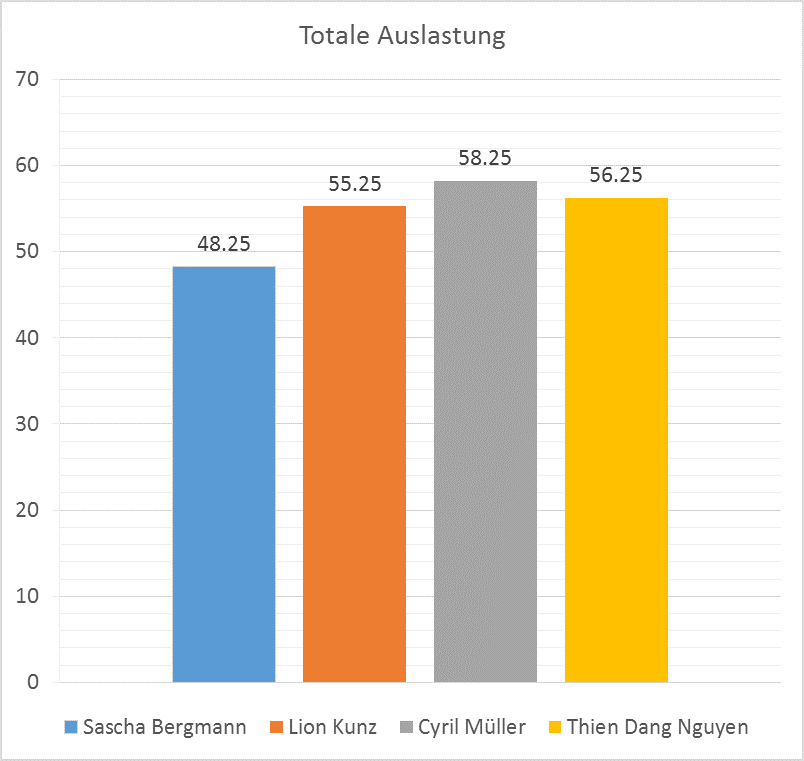
\includegraphics[width=0.7\textwidth]{graphics/auslastung_total.png}
\caption{Aufwand pro Person.}
\end{figure}

\appendix
\begin{landscape}
\section{Anhang}
\subsection{Arbeitspakete und Aufwandschätzung}
\begin{tabularx}{\linewidth}{|X|c|c|l|l|c|} \hline
\textbf{Arbeitspaket}&	\textbf{Aufwand Gesamt}&	\textbf{Aufwand/Person}&	\textbf{Verantwortlich}&	\textbf{Ausgeführt von}&	\textbf{Meilenstein}\\ \hline
UI-Design 																&	25	&	6,25&	Lion Kunz		&	Ganzes Team&	M1\\ \hline
Softwareentwurf															&	30	&	7,5	&	Cyril Müller	&	Ganzes Team&	M1\\ \hline
DB-Design																&	5	&	5	&	Sascha Bergmann	&	Cyril Müller&	M1\\ \hline
Java-Implementierung: Projekt und Grobstruktur, DB-Anbindung			&	10	&	10	&	Lion Kunz		&	Sascha Bergmann&	M2\\ \hline
Grundgerüst Web erstellen												&	6	&	6	&	Cyril Müller	&	Dang Thien Nguyen&	M2\\ \hline
UI erstellen für Login, Logout, Registrierung, Benutzer bearbeiten		&	6	&	6	&	Cyril Müller	&	Dang Thien Nguyen&	M2\\ \hline
UI erstellen für Datei hochladen, bearbeiten, anzeigen					&	8	&	8	&	Lion Kunz		&	Dang Thien Nguyen&	M2\\ \hline
Java-Implementierung: Login, Logout, Zugriffskontrolle					&	8	&	8	&	Dang Thien Nguyen&	Cyril Müller&	M2\\ \hline
Serverkonfiguration														&	3	&	3	&	Sascha Bergmann	&	Cyril Müller&	M2\\ \hline
Java-Implementierung: Dateifunktionen, Zugriff beantragen, freigeben	&	12	&	12	&	Dang Thien Nguyen&	Lion Kunz&	M2\\ \hline
\end{tabularx}
\clearpage
\begin{tabularx}{\linewidth}{|X|c|c|l|l|c|} \hline
\textbf{Arbeitspaket}&	\textbf{Aufwand Gesamt}&	\textbf{Aufwand/Person}&	\textbf{Verantwortlich}&	\textbf{Ausgeführt von}&	\textbf{Meilenstein}\\ \hline
UI erstellen für persönliche Startseite, Suchresultate					&	10	&	10	&	Cyril Müller	&	Dang Thien Nguyen&	M3\\ \hline
UI erstellen für Modul und Gruppen bearbeiten, erstellen, anzeigen		&	9	&	9	&	Sascha Bergmann	&	Lion Kunz&	M3\\ \hline
Java-Implementierung: Suche 											&	12	&	12	&	Lion Kunz		&	Sascha Bergmann&	M3\\ \hline
Java-Implementierung: Modulfunktionen 									&	8	&	8	&	Dang Thien Nguyen&	Cyril Müller&	M3\\ \hline
Java-Implementierung: Gruppe erstellen, bearbeiten, löschen 			&	8	&	8	&	Lion Kunz		&	Cyril Müller&	M3\\ \hline
Java-Implementierung: Benutzer erstellen und bearbeiten 				&	8	&	8	&	Cyril Müller	&	Lion Kunz&	M3\\ \hline
Test 																	&	30	&	7,5	&	Dang Thien Nguyen&	Ganzes Team&	M4\\ \hline
Reserve 																&	22	&	22	&	Sascha Bergmann	&	&	M4\\ \hline
Dokumentation 															&	20	&	5	&	Lion Kunz		&	Ganzes Team&	M4\\ \hline
\textbf{Total}																	&	\textbf{240}	&		&	&	&	\\ \hline
\end{tabularx}
\end{landscape}
\end{document}